\documentclass[]{report}

\voffset=-1.5cm
\oddsidemargin=0.0cm
\textwidth = 480pt

\usepackage{framed}
\usepackage{subfiles}
\usepackage{enumerate}
\usepackage{graphics}
\usepackage{newlfont}
\usepackage{eurosym}
\usepackage{amsmath,amsthm,amsfonts}
\usepackage{amsmath}
\usepackage{color}
\usepackage{amssymb}
\usepackage{multicol}
\usepackage[dvipsnames]{xcolor}
\usepackage{graphicx}
\begin{document}
	


\chapter{Session 7}

%------------------------------------%

\section*{Session 07:Sequences and Series}
\begin{itemize}
\item[7A.1] Sequences
\item[7A.2] Induction
\item[7A.3] Series and the Sigma Notation
\end{itemize}

\subsection*{Recurrence Relations(7.1.1)}



$u_1 = 2$
$u_2 = u_1 + 3 = 2 +3 = 5$
$u_3 = u_2 + 3 = 5+ 3 = 8$
Airthmetic Progression


\subsection*{Proof by Induction(7.2.2)}
\begin{itemize}
\item[Step 1] Base case
\item[Step 2] Induction hypothesis
\item[Step 3] Induction step
\end{itemize}



\subsection*{Series and Sigma Notation(7.2.3)}




Say which of the set the following numbers belong to.

If they belong to more than one of these sets, give all the sets.

$\sqrt{2}$
$\frac{3}{7}$

%------------------------------------------------------



\subsection*{Section 8 Exercises}
\begin{itemize}
\item $8^{\frac{1}{3}}$ Recall $a^{\frac{b}{c}} = a^{\frac{b}{c}}$
\item
\item
\end{itemize}



%------------------------------------%




%------------------------------------%
\subsection{Sequence and Series and Proof by Induction}


\[\sum^{n}_{i=1} (n^2) \]





\subsection{Question 10}

(a) Given the following adjacency matrices A and B where
A =

1 0 1
0 1 2
1 2 0

,B =

1 2 0
2 0 1
0 1 1

%MAKE NO

%--------------------------------------------%

(i) Say whether or not the graphs they represent are isomorphic.
(ii) Calculate A2 and A4 and say what information each gives about the graph
corresponding to A. [6]
(b) (i) Write down the augmented matrix for the following system of equations.

\[2x + y - z = 2\]
\[x - y + z = 4\]
\[x + 2y + 2z = 10\]
(ii) Use Gaussian elimination to solve the system. [4]


%--------------------------------------------%
\newpage
\chapter{Session 9}
\section{Probability and Counting}
%-------------------------------------------------------------------------%
\newpage

\textbf{Three Steps}
\begin{description}
\item[Step 1]
\item[Step 2]
\item[Step 3]
\end{description}


{Proof by Induction}

Let the summation $s_n$ be defined as follows:
\[s_n = 1 + 3 + 5 + \ldots + (2n - 1) \qquad \mbox{for n }\in \mathbb{Z}^{+}\]

Use the method of induction to prove that $s_n = n^2$ for all $n \geq 1$.


%------------------------------------------- %


%------------------------- %
% Section 1
\subsection{Axioms of Probability}

The Axioms of Probability

\begin{itemize}
\item The probability of a certain event is 1.
\item The probability of an impossible event is 0.
\item 
\end{itemize}
%------------------------- %
%-------------------------- %
\section*{Session 09: Probability}
\begin{itemize}
\item[9A.1] Counting Methods
\item[9A.2] Counting using Sets
\item[9A.3] Probability
\item[9A.4] Independent Events
\end{itemize}
\begin{itemize}
\item[9B.1] 


%-----------------------------------------------------%







%-----------------------------------------------------%



\section*{Question 10}

\subsection*{Session 10: Matrices and Systems of Equations}
\begin{itemize}
\item[10A.1] Dimensions of a Matrix
\item[10A.2] Matrix Multiplication
\item[10A.3] Matrix Calculations
\item[10A.4] 
\end{itemize}

\begin{itemize}
\item[10B.1] Systems of Equations
\item[10B.2] Expression Systems of Equations as Matrices
\item[10B.3] Augmented Matrices
\item[10B.4] Guassian Elimination
\end{itemize}
%-----------------------------------%
\subsection*{Question 10A}

Say what information the first row of the matrix contains.
Find the number of edges of G.


Write doen the augmented matrix for the following system of equations.
x+y+2z=7
2x+y+3z =11
x-27+5z=4


Use Gaussian elimination to solve the system.


\section{Matrices}

What are the dimensions of the following matrix


\[ \left(
\begin{array}{cc}
a_1 & a_2 \\ 
b_1 & b_2
\end{array} \right)\left(
\begin{array}{cc}
c_1 & d_1 \\ 
c_2 & d_2
\end{array} \right) = \left(
\begin{array}{cc}
(a_1 \times c_1) + (a_2 \times c_2) & (a_1 \times d_1) + (a_2 \times d_2) \\ 
(b_1 \times c_1) + (b_2 \times c_2) & (b_1 \times d_1) + (b_2 \times d_2)
\end{array} \right) \]

\bigskip
\large{
\[ \left(
\begin{array}{cc}
1 & 3 \\ 
0 & 2
\end{array} \right)\left(
\begin{array}{cc}
1 & 2 \\ 
4 & 1
\end{array} \right) = \left(
\begin{array}{cc}
(1 \times 1) + (3 \times 4) & (1 \times 2) + (3 \times 1) \\ 
(0 \times 4) + (2 \times 4) & (0 \times 2) + (2 \times 1)
\end{array} \right) = \left(
\begin{array}{cc}
14 & 5 \\ 
8 & 2
\end{array} \right) \]
}

\[ \left(
\left(
\begin{array}{cc}
1 & 2 \\ 
4 & 1
\end{array} \right)
\begin{array}{cc}
1 & 3 \\ 
0 & 2
\end{array} \right) = ? \]


%--------------------- %
% - 1.2 2010 
\begin{enumerate}[(i)]
\item
\end{enumerate}
%=====================================================================%
\subsection*{Question 4}
Let $S$ be the set of all 4 bit binary strings. The function $f : S \rightarrow Z$
is defined by the rule:
\[f(x) = \mbox{ the number of zeros in x} \] for each binary string $x \in S$.
Find:
\begin{itemize}
\item[(a)] (4 Marks) Answer the following questions
\begin{itemize}
\item[(i)] the number of elements in the domain
\item[(ii)] f(1010)
\item[(iii)] the set of pre-images of 1
\item[(iv)] the range of f. 
\end{itemize}
\item[(b)] (2 Marks) Decide whether the function $f$, as defined above, has either the one to one or
the onto property, justifying your answers. 
\item[(c)] (2 Marks) State the condition to be satisfied by a function $f : X \rightarrow Y$ for it to have an
inverse function $f^{-1} : Y \rightarrow X$.
\item[(d)] (2 Marks) Define the inverse functions for each of the following:
\end{itemize}
%---------------------------------------------------------%
%\section*{Question 5}
%
%\begin{figure}
%\centering
%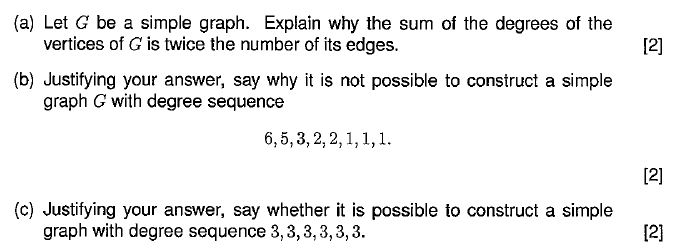
\includegraphics[width=0.7\linewidth]{GraphTheoryQuestion2012}
%
%\end{figure}


%----------------------------------------------------------------%
\newpage
\section*{Question 6}
% 2007 Q8
Given a flock of chickens, between any two chickens one of them is
dominant. A relation, R, is defined between chicken x and chicken y as xRy if x is
dominant over y. This gives what is known as a pecking order to the flock. Home
Farm has 5 chickens: Amy, Beth, Carol, Daisy and Eve, with the following relations:

\begin{itemize}
\item Amy is dominant over Beth and Carol
\item Beth is dominant over Eve and Carol
\item Carol is dominant over Eve and Daisy
\item Daisy is dominant over Eve, Amy and Beth
\item Eve is dominant over Amy.
\end{itemize}

\newpage
\section*{Question 6}
% Digraphs and Relations
% http://staff.scem.uws.edu.au/cgi-bin/cgiwrap/zhuhan/dmath/dm_readall.cgi?page=20



%============================================================================%




\newpage
%===========================================================%
\section*{Question 10}
%%--------------------------------------------%
%\noindent \textbf{Part A : Matrix Operations - 4 Marks}\\ 
%\begin{figure}[h!]
%\centering
%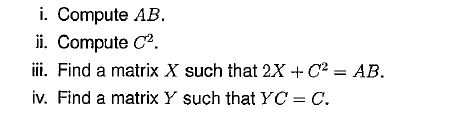
\includegraphics[width=1.11\linewidth]{MatrixQuestion2012}
%
%\end{figure}


%--------------------------------------------%
\noindent \textbf{Part B : Gaussian Elimination - 5 Marks}\\ 
\begin{itemize}
\item[(i)] Say whether or not the graphs they represent are isomorphic.
\item[(ii)] Calculate $A^2$ and $A^4$ and say what information each gives about the graph
corresponding to A. [6]
\end{itemize}
%===========================================%
\begin{itemize}
\item[(i)] Write down the augmented matrix for the following system of equations.
\[2x + y - z = 2\]
\[x - y + z = 4\]
\[x + 2y + 2z = 10\]
\item[(ii)] Use Gaussian elimination to solve the system. 
\end{itemize}
%=========================================================================================== %


%-------------------------------------------------------------------------%
\newpage

\end{document}
